%% ============================================================================
%% ============================================================================
\section{The Impossibility Bound}
\label{sec:ident}

The estimator is pure accounting and uses neither a run threshold nor
any fitted parameter. Let $\phi$ be the fraction of reserves impaired and $\rho\in[0,1]$ the
expected recovery rate on the impaired assets. The fraction permanently lost is
$\phi(1-\rho)$, so the no-panic price floor, expected backing per coin, is
\begin{equation}
P_{\mathrm{fund}} = 1 - \phi(1-\rho).
\label{eq:floor}
\end{equation}

\subsection{Assumptions}
The bound rests on three assumptions, and a fourth serves Corollary~\ref{cor:fosd}.
\begin{description}
\item[(A1) Reserve-only fundamental.] A coin's fundamental value is its expected reserve
  backing per unit given \emph{disclosed} reserves. The only impairment is the exposure $\phi$.
\item[(A2) Par redemption when solvent.] Conditional on rescue, redemption is at \$1
  \emph{within the analysis horizon}.
\item[(A3) Bounded recovery.] Recovery on impaired reserves satisfies $\rho\in[0,1]$ because
  the coin is fully reserved and the reserves carry no leverage, so the worst case is total permanent
  loss of the impaired fraction.
\item[(A4) Monotone-utility valuation.] The unconstrained marginal holder values the claim as
  an expected utility of its payoff, for \emph{some} monotone increasing utility and
  \emph{some} probability measure over outcomes, with no ambiguity about the disclosed $\phi$.
  This nests risk neutrality, any degree of risk aversion, and rank-dependent weighting.
\end{description}

The closing clause of (A4) assumes away ambiguity about the disclosed $\phi$. The $12.3\%$
margin is the principal defense against it, and the $\phi$-by-feed grid of
Section~\ref{sec:sensitivity} is the second: a holder who doubted the disclosure would have to
price an impairment $4.3$ points above the disclosed figure with zero recovery before the
trough becomes rationalizable.

\subsection{Statement and proof}
Under (A1)--(A3), take a pricing measure under which the impaired fraction's loss goes
\emph{unremediated} with probability $q\in[0,1]$. Remediation here means an issuer
make-whole, a deposit-insurance recovery, or an official backstop. The expected-loss price is
\begin{equation}
P_{\mathrm{fund}}(q,\rho) = 1 - q\,\phi\,(1-\rho).
\label{eq:plossq}
\end{equation}
This is the standard floor-at-recovery-value bound of credit pricing: risky debt is bounded
below by its recovery value under any pricing measure~\cite{merton1974}, with $q$ a
reduced-form failure intensity~\cite{duffiesingleton1999}.

\begin{proposition}[Rational-pricing floor and impossibility]
\label{prop:floor}
Under \textup{(A1)--(A3)}, $P_{\mathrm{fund}}(q,\rho)\in[\,1-\phi,\;1\,]$ for all
$q,\rho\in[0,1]$. Hence any observed price $P_{\mathrm{obs}}<1-\phi$ cannot be rationalized as
expected loss. The unremediated-loss probability it would require, at the worst-case recovery
$\rho=0$, is
\begin{equation}
q^\star = \frac{1-P_{\mathrm{obs}}}{\phi} \;>\;1 .
\end{equation}
Equivalently, the price is unrationalizable for any impairment $\phi<1-P_{\mathrm{obs}}$.
\end{proposition}

\begin{proof}
In \eqref{eq:plossq}, $P_{\mathrm{fund}}$ is decreasing in $q$ and increasing in $\rho$ on
$[0,1]^2$. It is therefore minimized at $(q,\rho)=(1,0)$, where it equals $1-\phi$, and
maximized at $q=0$ or at $\rho=1$, where it equals $1$. Thus $P_{\mathrm{fund}}\in[1-\phi,1]$.
If $P_{\mathrm{obs}}<1-\phi$,
no $(q,\rho)\in[0,1]^2$ solves $P_{\mathrm{obs}}=P_{\mathrm{fund}}(q,\rho)$. Setting $\rho=0$
and solving $P_{\mathrm{obs}}=1-q\phi$ gives $q^\star=(1-P_{\mathrm{obs}})/\phi$, which
exceeds $1$ exactly when $P_{\mathrm{obs}}<1-\phi$, i.e.\ $\phi<1-P_{\mathrm{obs}}$. \qed
\end{proof}

The proof never restricts $q$ to a physical probability, so it covers any
risk-neutral pricing measure. Under \textup{(A1)--(A4)} the floor is preference-free:

\begin{corollary}[Preference-free floor for rational valuations]
\label{cor:fosd}
Under \textup{(A1)--(A4)}, the payoff on a USDC claim has support in $[\,1-\phi,\;1\,]$, and
for any monotone increasing utility $u$ and any probability measure over outcomes, the
certainty equivalent $u^{-1}\!\bigl(\mathbb{E}[u(X)]\bigr)$ of a payoff lottery $X$ with
support in $[1-\phi,1]$ itself lies in $[1-\phi,1]$. No rational valuation, under any
monotone increasing utility and given the support bound, falls below $1-\phi$. A more
risk-averse holder values the claim lower within the band, but never below $1-\phi$.
\end{corollary}

\begin{proof}
By (A2)--(A3) the payoff satisfies $X\in[1-\phi,1]$ in every state. Monotonicity gives
$u(X)\ge u(1-\phi)$ pointwise, hence $\mathbb{E}[u(X)]\ge u(1-\phi)$. Applying the
increasing function $u^{-1}$ yields a certainty equivalent of at least $1-\phi$. The upper
edge is symmetric. This is first-order stochastic dominance over a bounded support and is
independent of the curvature of $u$. \qed
\end{proof}

Two distinctions govern the Corollary's interpretation. First, it bounds rational
\emph{valuations}, meaning willingness to pay, and not market-clearing \emph{prices}. Under
binding margin or capital constraints, a forced seller can rationally transact below every
unconstrained valuation. This is the classic limits-to-arbitrage
mechanism~\cite{shleifervishny1997,grombvayanos2010}. That channel is a friction, so it lies
inside the non-fundamental share $s_{\mathrm{nf}}$ of \eqref{eq:share}. Second, the floor
is as strong as the support bound $X\in[1-\phi,1]$ and no stronger. \emph{Issuer-wrapper risk} is not covered by that bound. This is an issuer insolvency that delivers
less than the floor, or delivers it late, through claim-priority uncertainty, administrative
cost, or a gated distribution~\cite{Gorton_2021}. (A1) prices that channel at zero, on three
facts. $77\%$ of reserves sat in a segregated, SEC-registered government money-market
fund custodied at BNY Mellon, not issuer-balance-sheet deposits~\cite{circle2023update}. A distribution delay is a
fundamental discount only through time value, and at 2023-03-10 Treasury yields
($4.81$--$5.01\%$)~\cite{ustreasury2023daily} a $\sim\!350$-day gate would be needed to reach
the trough from the floor. Wrapper costs alone would need a $4.3$-point ($12.3-8.0$) loss on
that money-market portfolio, and no segregated government-fund structure has recorded such a
loss. The floor is therefore conditional on (A1)'s disclosed-impairment support, leaving only
a marketability discount that scales with \emph{ex-ante} volatility, small relative to
realized crisis volatility for short-dated Treasuries and cash~\cite{longstaff1995}.

\subsection{Application to the March 2023 USDC trough}
With the disclosed impairment $\phi=0.08$, the floor is $1-\phi=\$0.92$. The observed trough
is $P_{\mathrm{obs}}=\$0.877$. Prose rounds the trough to three figures throughout, while
every quantity computed at the trough is evaluated on the frozen four-figure print,
\$0.8767, so \$0.877 and \$0.8767 denote one reading. The trough lies below the \$0.92 floor.
The implied unremediated-loss probability is
\begin{equation}
q^\star = \frac{1-0.877}{0.08} = 1.54 \;>\;1 .
\end{equation}
No admissible $(q,\rho)$ rationalizes the trough, so the de-peg is non-fundamental by impossibility, not by assumption.
The timing makes the bound conservative. The trough
precedes Circle's make-whole pledge by at most $12.5$ hours and precedes the federal joint
statement by $38.3$ hours (22:15~UTC, 12~March~2023)~\cite{fedtreasfdic2023pressrelease}. The
pledge carries no publication timestamp, so the $12.5$-hour figure is measured to its first
web-archive capture, 20:27~UTC on 11~March~2023~\cite{circle2023update}. The floor requires
no backstop concept, only that the payoff cannot fall below $1-\phi$ state by state.
Neither the trough reading nor the reserve denominator moves the conclusion, because the
margin between the floor and the trough is wide relative to the variation in either. At the composite trough
(\$0.8767) the lower edge of \eqref{eq:share} is $35.1\%$. At the deepest USDT-denominated
Binance hourly low (\$0.882) it is $32.2\%$. At the next-lowest composite hourly print
(\$0.8949) it is $23.9\%$.
At Circle's alternate $\sim\$42.1$B reserve-composition total ($\phi=7.84\%$) the lower edge
is $36.4\%$. At the disclosed $\sim\$40$B total ($\phi=8\%$, the headline used throughout) it is $35.1\%$. At the precise \$3.3B/\$40.0B ratio ($\phi=8.25\%$) it is
$33.1\%$, a $7.8$--$8.3\%$ band across the three denominators, and a larger reserve total
only shrinks $\phi$ and widens the margin by which the trough is unrationalizable. Over the
same three denominators the implied $q^\star$ ranges from $1.49$ to $1.57$, against the
headline $q^\star=1.54$ at $\phi=0.08$.

\begin{figure}[t]
\centering
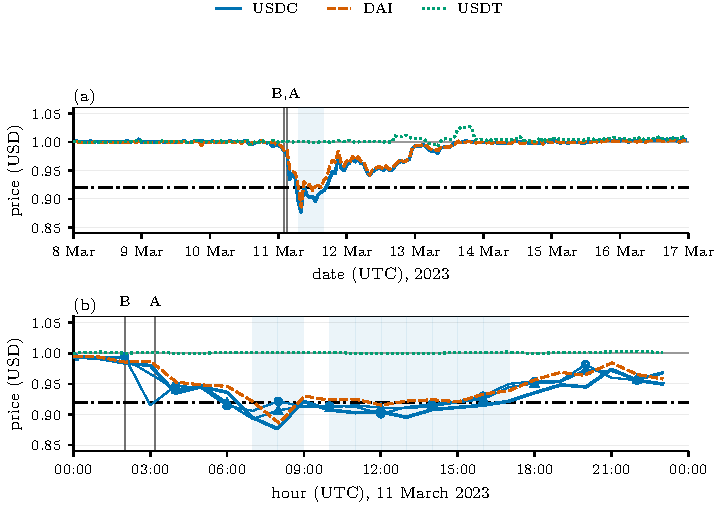
\includegraphics[width=\textwidth]{figs/fig_event.pdf}
\caption{Hourly USD prices of USDC (solid), DAI (dashed), and USDT (dotted) over the
analysis window (a) and over 11~March 2023 (b), against par and the \$0.92 floor implied
by Circle's disclosed $\phi=0.08$. Hatched columns in (b) are USDC's nine breaching hours,
06{:}59--16{:}00 UTC, and the unhatched column is the recovery hour. Vertical lines mark
A, Circle's disclosure (03:11 UTC, 11~March), and B, the Coinbase USDT-USD premium peak
(02:00 UTC, 11~March).}
\label{fig:event}
\end{figure}

\paragraph{Hourly evaluation of the bound.}
Because the estimator requires only a price and a publicly quantified $\phi$, it can be evaluated at
every hour of the frozen window (Figure~\ref{fig:event}). Of USDC's $212$ in-window
hourly readings, $9$ lie below the \$0.92 floor. All nine fall on 11~March 2023, between
06{:}59 and 16{:}00~UTC, opening at $q^\star=1.31$ and peaking an hour later at the
trough. Over the same window, DAI breaches in $2$ of $214$ hours and USDT in
none of $213$ (Table~\ref{tab:firing}).
\emph{This is duration and specificity, not evidence volume:} hourly prices within one
episode are near-unit-root (lag-1 autocorrelation $0.963$), so the $212$ readings carry an
AR(1)-adjusted effective sample size of $4.0$, and identification still rests on one
episode and one disclosed $\phi$.

\subsection{The non-fundamental share}
Write the observed deviation $\Delta_{\mathrm{obs}}=1-P_{\mathrm{obs}}$ and the fundamental
deviation $\Delta_{\mathrm{fund}}=\phi(1-\rho)$. The non-fundamental share of the de-peg is
\begin{equation}
s_{\mathrm{nf}}(\rho) = \frac{\Delta_{\mathrm{obs}}-\Delta_{\mathrm{fund}}}{\Delta_{\mathrm{obs}}}
= \frac{(1-P_{\mathrm{obs}})-\phi(1-\rho)}{1-P_{\mathrm{obs}}} .
\label{eq:share}
\end{equation}
Two independent restrictions give the band edges. The \emph{lower edge} ($\rho=0$) takes even
a total permanent loss of the impaired reserves as the fundamental cap. At $\phi=0.08$,
$s_{\mathrm{nf}}(0)=(0.1233-0.08)/0.1233=0.351\approx 35\%$. The \emph{upper edge} ($\rho=1$)
uses the full re-peg, which implies no permanent loss occurred, so $\Delta_{\mathrm{fund}}=0$
and $s_{\mathrm{nf}}(1)=1$: $100\%$ ex post, an identity. This upper edge is a realized-loss
identity, not an expected-loss bound. It substitutes the observed outcome, full recovery and
therefore zero permanent loss, for an expectation over $\rho$, so it is an ex-post statement.
The $\rho=0$ lower edge is the ex-ante worst-case expectation. We report the band
$[35\%,100\%]$. The full re-peg supports the high end of that band. ``Non-fundamental'' means
coordination panic \emph{plus} microstructure friction, so the share is an upper bound on pure
coordination panic.

Four quantities in this paper are one quantity presented four ways. $q^{\star}$,
$s_{\mathrm{nf}}(0)$, the margin column of Table~\ref{tab:panel}, and the floor-breach
indicator are all determined by $1-P_{\mathrm{obs}}-\phi$, so agreement among them
corroborates nothing.

\subsection{Robustness to $\phi$ and to the assumptions}
The lower edge depends on $\phi$.
By Proposition~\ref{prop:floor}, the trough is unrationalizable for any
$\phi<1-P_{\mathrm{obs}}=0.123$, i.e.\ for any impairment below $12.3\%$, a $4.3$-point
margin over the disclosed $8\%$. The non-fundamental share's lower edge ($\rho=0$) varies
with $\phi$ but stays strictly positive throughout this margin, falling to
$\approx 19\%$ at $\phi=0.10$.

(A1) is the binding assumption. If a coin carried fundamental value beyond disclosed
reserves, the floor would shift. For that reason $\phi$ is taken from Circle's disclosure
rather than fitted, and we report a band. Three further checks discipline
(A1). First, the exact denominator is immaterial, as the sensitivity above shows. Second, the par-safety of
the non-SVB reserves rests on Circle's audited attestation, which itemizes them at the CUSIP
level. They are ${\sim}\$38.5$B of short-dated U.S. Treasuries plus cash.
The attestation shows reserves exceeding USDC in circulation on both its March report dates,
and the failed banks no longer appear in the March~31
schedule~\cite{circle2023attestation}.
Third, the contagion-week worst case is bounded \emph{ex ante}: at the trough, $77\%$ of
reserves (\$32.4B) were short-dated Treasuries in the segregated, BNY-Mellon-custodied Circle
Reserve Fund, and the \$9.7B cash leg was held at several
institutions, of which SVB was one~\cite{circle2023update}. Raising $\phi$ past $12.3\%$ would require zero-recovery
losses on more than \$5.2B of reserves, taken against Circle's \$42.1B reserve-composition
total: writing off SVB's \$3.3B and \$1.9B of the \$6.4B cash leg held elsewhere, since
the leg is \$9.7B less the \$3.3B at SVB and the threshold is \$5.2B less that same
\$3.3B. No U.S. resolution on record has produced that outcome.

(A2)--(A3) are conservative: par redemption and bounded recovery both \emph{raise} the
floor, so relaxing them cannot weaken the lower edge. (A4) is dispensable for
Proposition~\ref{prop:floor}: it is used only by Corollary~\ref{cor:fosd}.
% Source: results/phi_denominator_sensitivity.json grid[] -- entries with
%   trough_label="composite_min_headline" at phi_label in {static_phi_altreserve_42.1B_0.0784,
%   static_phi_svb_0.08, static_phi_3.3_over_40.0_0.0825}: q_star_rho0 = 1.573 / 1.5416 / 1.4948
%   respectively. The rho=1 identity is rational_bound.py's own stated pricing relation
%   P_fund(q,rho) = 1 - q*phi*(1-rho) (module docstring + implied_failure_prob's denominator
%   phi*(1-rho_fail), which vanishes at rho=1 for any phi>0, making P_fund identically 1 for
%   every admissible q). This sentence
%   supplements Proposition 1 / Corollary 1 rather than replacing their formal statements.
Under the worst-case recovery assumption $\rho=0$, the implied unremediated-loss probability at
the composite trough exceeds the admissible $[0,1]$ range at every $\phi$ in the sensitivity
grid: $q^{\star}=1.57$ at $\phi=0.0784$, $q^{\star}=1.54$ at $\phi=0.08$, and $q^{\star}=1.49$ at
$\phi=0.0825$. At the opposite extreme, $\rho=1$ collapses the pricing relation to the identity
$P_{\mathrm{fund}}(q,1)=1-q\phi(1-1)\equiv 1$ for every $q\in[0,1]$, so full assumed recovery
makes the floor coincide with par and the bound uninformative. This is why
Proposition~\ref{prop:floor} and
Corollary~\ref{cor:fosd} are evaluated at $\rho=0$ throughout.

